\documentclass{beamer}
\usetheme{Berlin}

\title{A Retrospective look on the 2024 Neural Networks-Deep Learning Assignments}
\author{Papadakis Konstantinos Fotios}
\date{\today}

\begin{document}
% Title Page
\frame{\titlepage}

% Frame 1: Algorithms
\begin{frame}
\frametitle{Different Algorithms}
We implement the following algorithms to solve our CIFAR-10 classification problem:
\begin{itemize}
\item K-Nearest Neighbors
\item Nearest Centroid
\item Convolutional Neural Network (CNN)
\item Multi-Layer Perceptron (MLP)
\item Support Vector Machine (SVM)
\end{itemize}
We will compare them with each other while explaining the way they work. We will also 
be mentioning some extra 
\end{frame}

% Frame 2: Dataset
\begin{frame}
    \frametitle{Dataset}
    We chose to go with CIFAR-10. A dataset which sports:
    \begin{itemize}
        \item 60,000 32x32 color images
        \item 10 classes, with 6,000 images per class
        \item 50,000 training images 
        \item 10,000 test images
    \end{itemize}
    The simplest algorithms we tried training the dataset on were K-Nearest Neighbors and 
    Nearest Centroid. Let's see them in greater detail.
\end{frame}

% Frame 3: CIFAR-10 Visualization
\begin{frame}
    \frametitle{CIFAR-10 Visualization}
    \begin{figure}
        \centering
        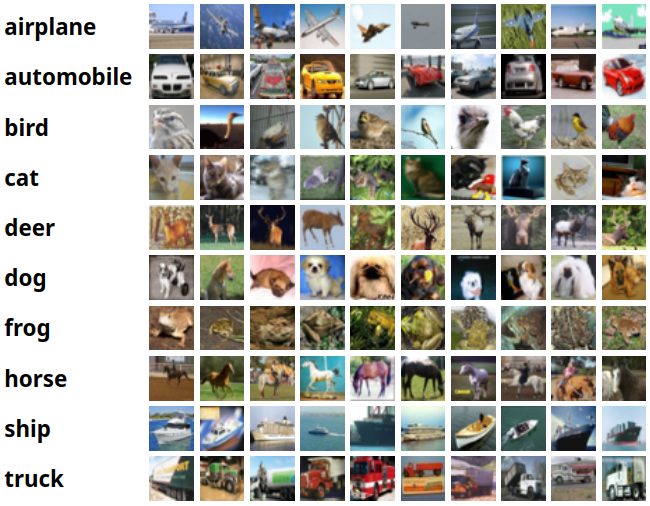
\includegraphics[width=0.6\textwidth]{media/cifar10_example.png}
        \caption{CIFAR-10 Dataset}
    \end{figure}
\end{frame}

% Frame 4: K-Nearest Neighbor
\begin{frame}
\frametitle{K Nearest Neighbor}
\begin{center}
    How does it work?
\end{center}
\begin{columns}
    \begin{column}{0.5\textwidth}
        We calculate the distance between each point in the test dataset with all the point from
        the training dataset. We then select the k-nearest points and classify the test point.
    \end{column}

    \begin{column}{0.45\textwidth}
        \begin{figure}
            \centering
            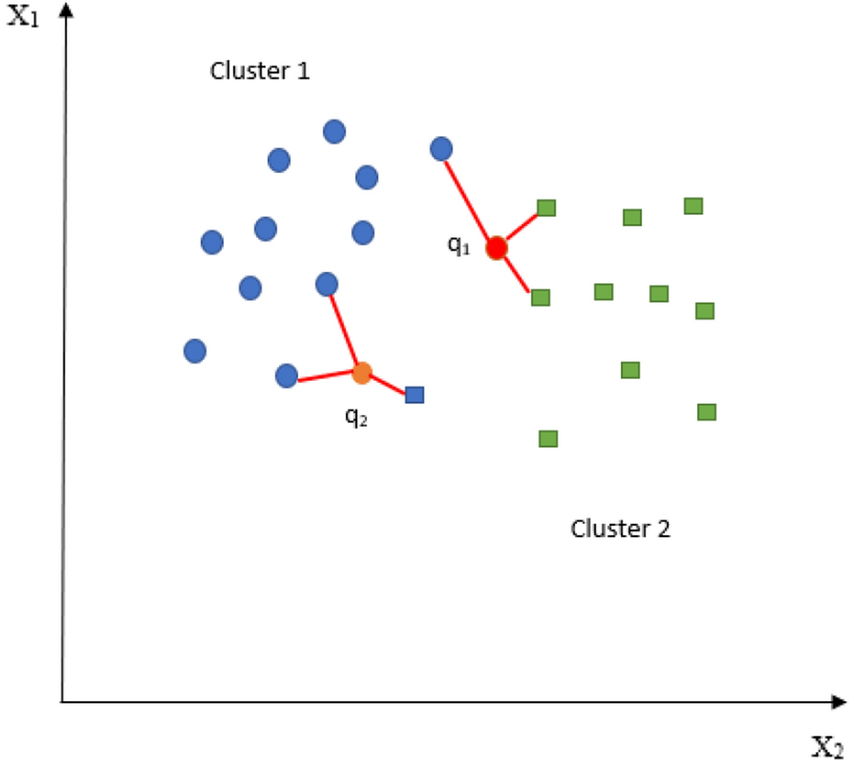
\includegraphics[width=1\textwidth]{media/knn_example.png}
            \caption{K-Nearest Neighbors}
        \end{figure}
    \end{column}
\end{columns}
\end{frame}

% Frame 5: Nearest Centroid
\begin{frame}
\frametitle{Nearest Centroid}
\begin{center}
    How does it work?
\end{center}

\begin{columns}
    \begin{column}{0.5\textwidth}
        We calculate the centroid of each class in the training dataset and then compare the 
        distance of the test point with each centroid. We classify the test point to the class
        with the closest centroid.
    \end{column}

    \begin{column}{0.5\textwidth}
        \begin{figure}
            \centering
            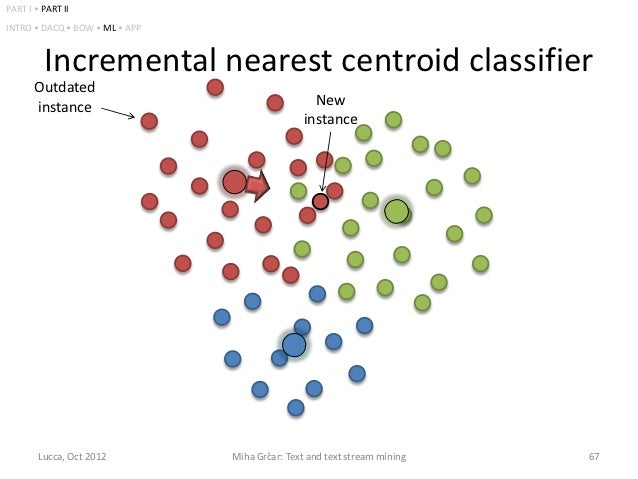
\includegraphics[width=1\textwidth]{media/centroid_example.jpg}
            \caption{Nearest Centroid}
        \end{figure}
    \end{column}
\end{columns}

\end{frame}

% Frame 6: Convolutional Neural Network
\begin{frame}
\frametitle{Convolutional Neural Network}
It is the first complex algorithm we tried. Here are the network characteristics we stuck to:
\begin{columns}
    \begin{column}{0.5\textwidth}
        \begin{itemize}
            \item 6 Convolutional Layers
            \item 3 Max Pooling Layers
            \item 2 Fully Connected Layers
            \item 1 Output Layer
            \item ReLU Activation Function
            \item Adam Optimizer
            \item Cross Entropy Loss
            \item Reduce Learning Rate on Plateau
        \end{itemize}
    \end{column}
    \begin{column}{0.5\textwidth}
        \begin{itemize}
            \item Dataset transformations such as:
            \begin{itemize}
                \item Random Horizontal Flip
                \item Random Rotation
                \item Random Crop    
            \end{itemize}
            \item Normalization around 0.5 for the mean and 0.2 for the standard deviation
        \end{itemize}
    \end{column}
\end{columns}
\end{frame}


\begin{frame}
\frametitle{Manual Testing Script}
\begin{columns}[t]
    \begin{column}{0.5\textwidth}    
        Custom script aiming to test performance on non-CIFAR-10 images.\\
        Options include testing on:
        \begin{itemize}
            \item A Random Image
            \item A Random CIFAR-10 Image
            \item A Batch of Random Images
        \end{itemize}
        On the right we can see an example output of the script.
    \end{column}

    \begin{column}{0.5\textwidth}
        \begin{figure}
            \centering
            \vspace{-1cm}
            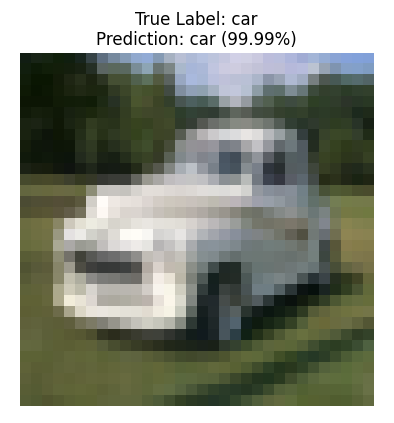
\includegraphics[width=0.9\textwidth]{media/random_cifar.png}
            \vspace{-0.3cm}
            \caption{A Random CIFAR-10 Image: Example Output}
        \end{figure}
    \end{column}
\end{columns}
\end{frame}

\begin{frame}
    \frametitle{Additional Testing Example}
    \begin{figure}
        \centering
        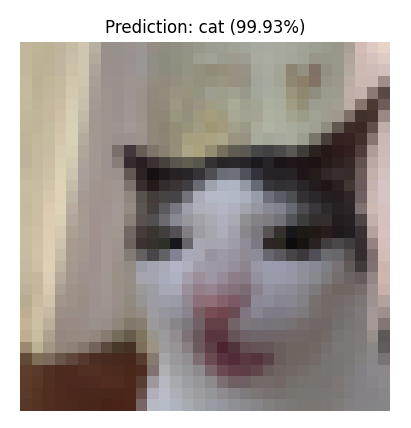
\includegraphics[height=0.7\textheight]{media/custom_image.png}
        \vspace{-0.3cm}
        \caption{A Random Image: Example Output}
    \end{figure}
\end{frame}

\begin{frame}
\frametitle{Manual Testing Results}
\begin{columns}
    \begin{column}{0.5\textwidth}
        \begin{figure}
            \centering
            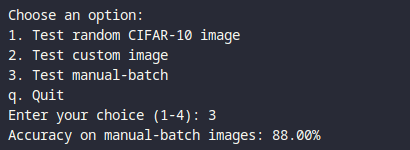
\includegraphics[width=1\textwidth]{media/manual_batch.png}
            \caption{Manual Testing Results}
        \end{figure}
    \end{column}

    \begin{column}{0.5\textwidth}
        Observations:
        \begin{itemize}
            \item Slightly worse performance 
            \item Not much over-fitting
        \end{itemize}
    \end{column}
\end{columns}
\end{frame}

\begin{frame}
\frametitle{Modifications}
We tried changing the following parameters:
\begin{itemize}
    \item Architecture
    \item Optimizer
    \item Normalization values
    \item Activation Function
\end{itemize}
\end{frame}

\begin{frame}
\frametitle{CNN vs MLP}
\begin{columns}
    \begin{column}{0.5\textwidth}
        \begin{figure}[t]
            \centering
            \vspace{-0.4cm}
            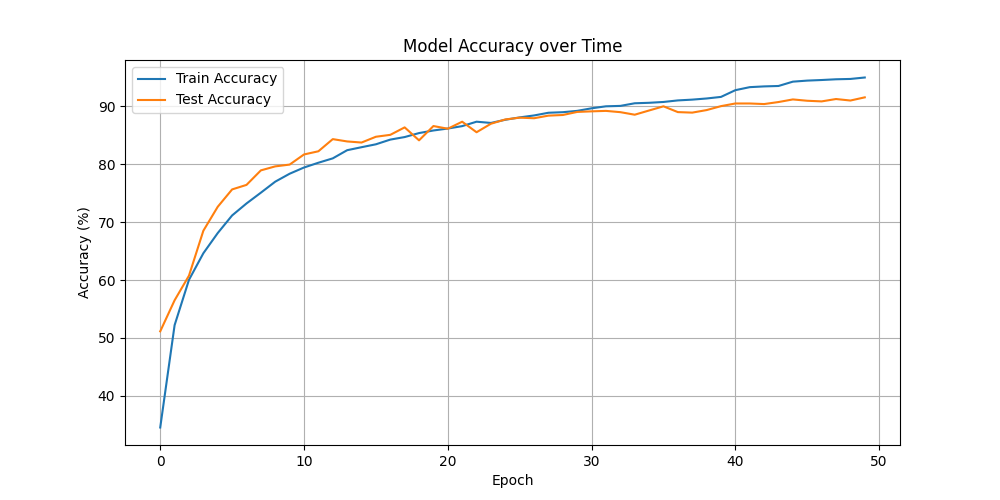
\includegraphics[width=0.9\textwidth]{media/cifar10_cnn_accuracy.png}
        \end{figure}
        \vspace{-0.8cm}
        \begin{figure}[t]
            \centering
            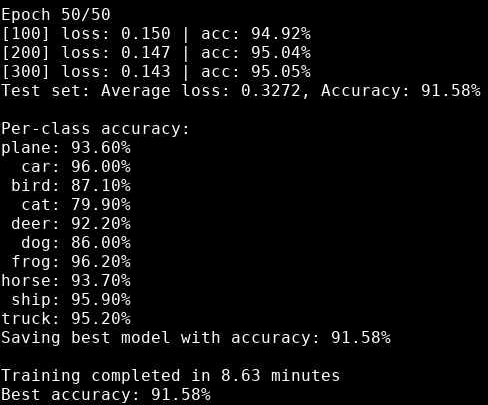
\includegraphics[width=0.9\textwidth]{media/cnn_epoch_50.png}
            \vspace{-0.3cm}
            \caption{CNN: Last Epoch}
        \end{figure}
    \end{column}

    \begin{column}{0.5\textwidth}
        \begin{figure}[t]
            \centering
            \vspace{-0.4cm}
            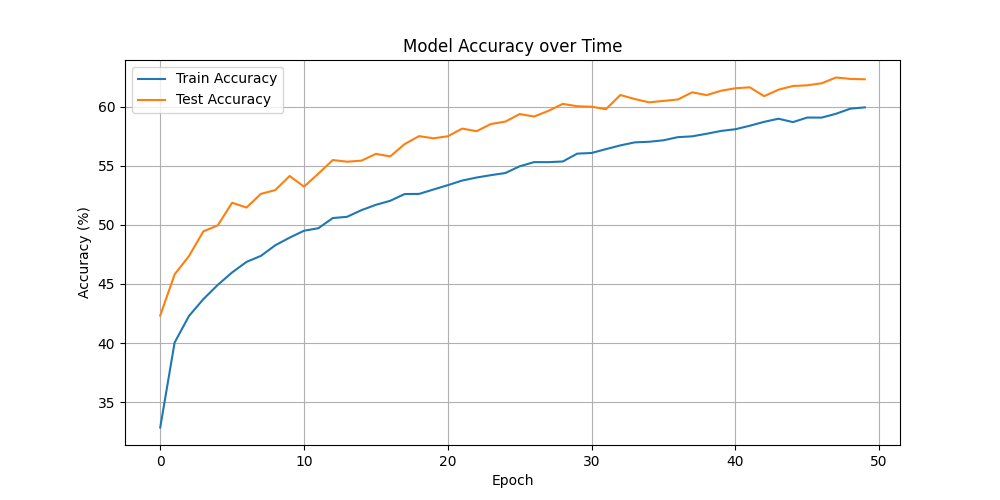
\includegraphics[width=0.9\textwidth]{media/cifar10_mlp_accuracy.png}
        \end{figure}
        \vspace{-0.8cm}
        \begin{figure}[t]
            \centering
            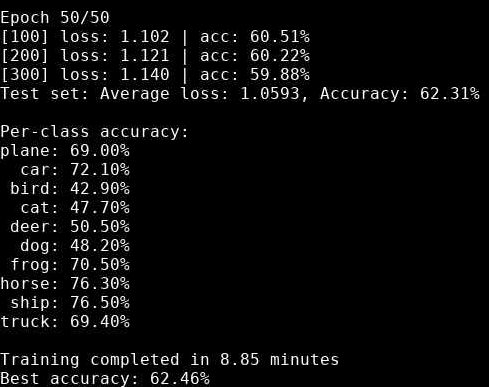
\includegraphics[width=0.9\textwidth]{media/mlp_epoch_50.png}
            \vspace{-0.3cm}
            \caption{MLP: Last Epoch}
        \end{figure}
    \end{column}
\end{columns}
\end{frame}

\begin{frame}
\frametitle{ReLU vs Tanh}
\begin{columns}
    \begin{column}{0.5\textwidth}
        \begin{figure}[t]
            \centering
            \vspace{-0.4cm}
            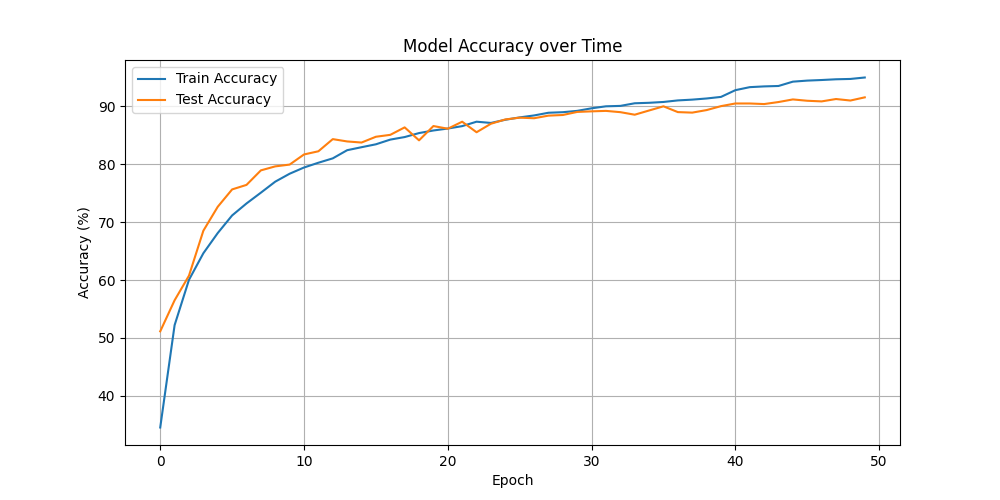
\includegraphics[width=0.9\textwidth]{media/cifar10_cnn_accuracy.png}
        \end{figure}
        \vspace{-0.8cm}
        \begin{figure}[t]
            \centering
            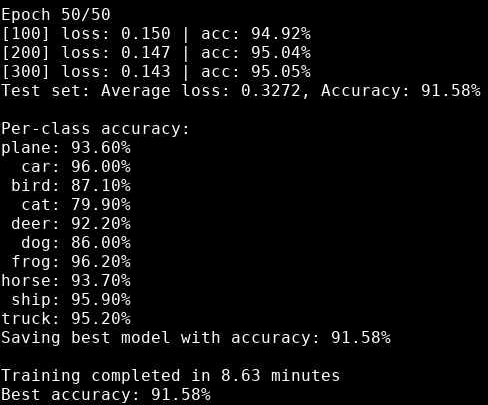
\includegraphics[width=0.9\textwidth]{media/cnn_epoch_50.png}
            \vspace{-0.3cm}
            \caption{ReLU: Last Epoch}
        \end{figure}
    \end{column}

    \begin{column}{0.5\textwidth}
        \begin{figure}[t]
            \centering
            \vspace{-0.4cm}
            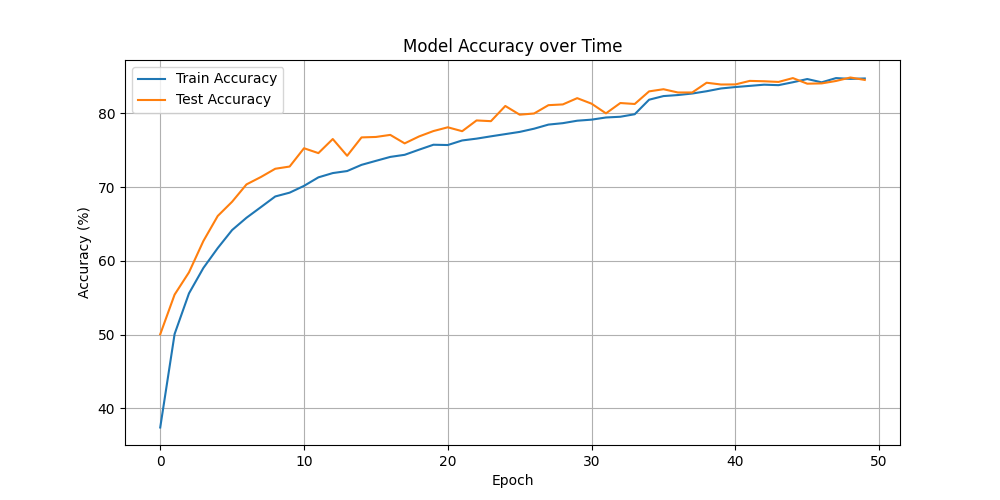
\includegraphics[width=0.9\textwidth]{media/cifar10_cnn_tanh_accuracy.png}
        \end{figure}
        \vspace{-0.8cm}
        \begin{figure}[t]
            \centering
            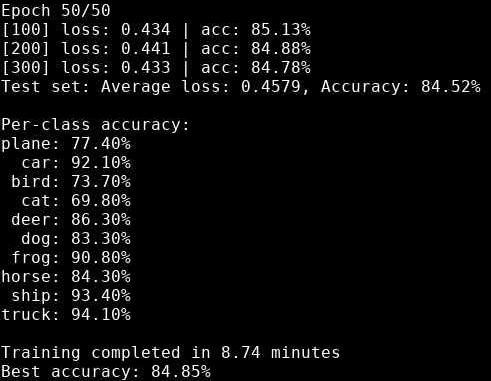
\includegraphics[width=0.9\textwidth]{media/cnn_tanh_epoch_50.png}
            \vspace{-0.3cm}
            \caption{Tanh: Last Epoch}
        \end{figure}
    \end{column}    
\end{columns}
\end{frame}

\begin{frame}
\frametitle{Adam vs SGD}
\begin{columns}
    \begin{column}{0.5\textwidth}
        \begin{figure}[t]
            \centering
            \vspace{-0.4cm}
            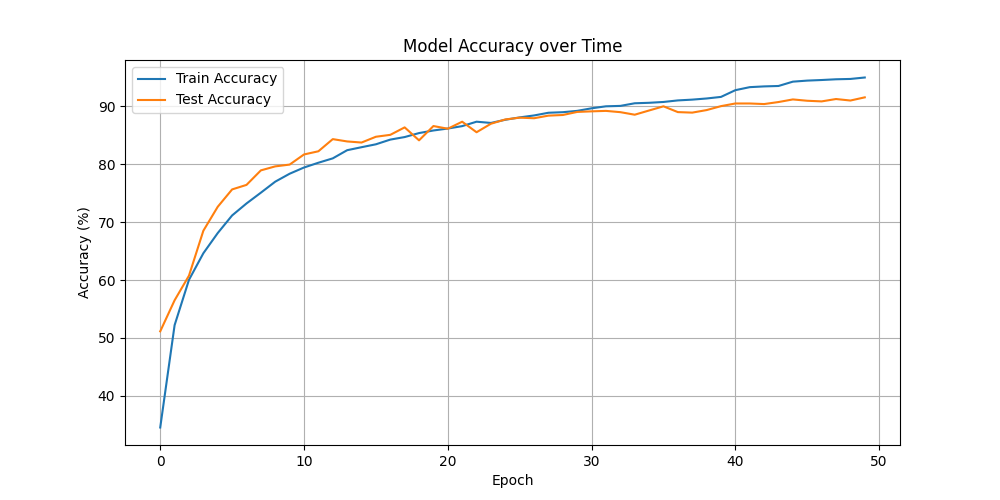
\includegraphics[width=0.9\textwidth]{media/cifar10_cnn_accuracy.png}
        \end{figure}
        \vspace{-0.8cm}
        \begin{figure}[t]
            \centering
            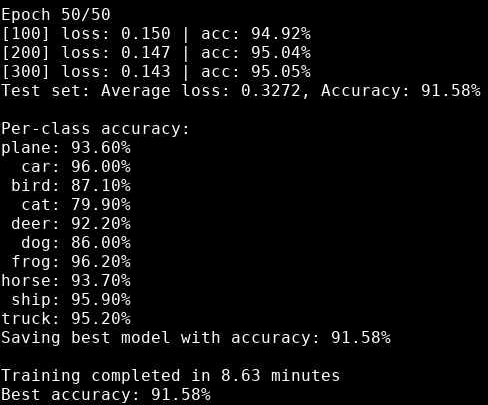
\includegraphics[width=0.9\textwidth]{media/cnn_epoch_50.png}
            \vspace{-0.3cm}
            \caption{Adam: Last Epoch}
        \end{figure}
    \end{column}

    \begin{column}{0.5\textwidth}
        \begin{figure}[t]
            \centering
            \vspace{-0.4cm}
            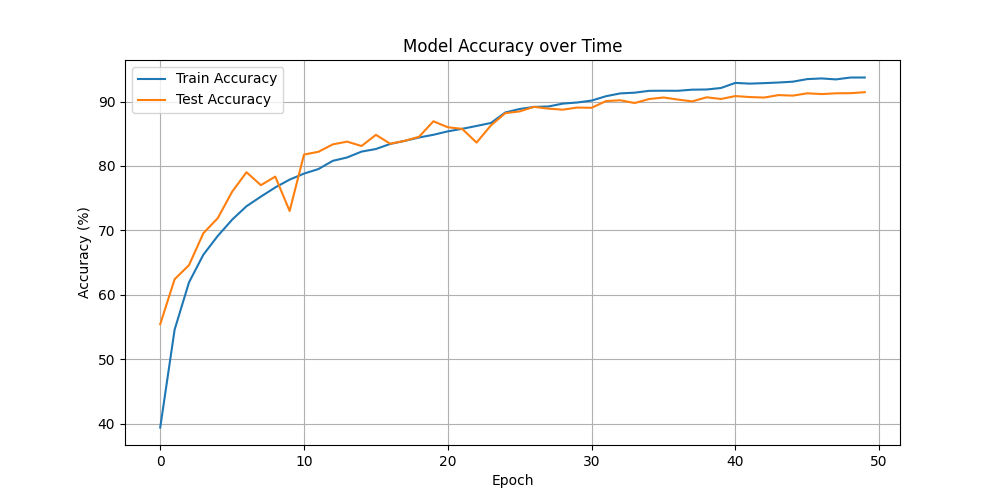
\includegraphics[width=0.9\textwidth]{media/cifar10_cnn_sgd_accuracy.png}
        \end{figure}
        \vspace{-0.8cm}
        \begin{figure}[t]
            \centering
            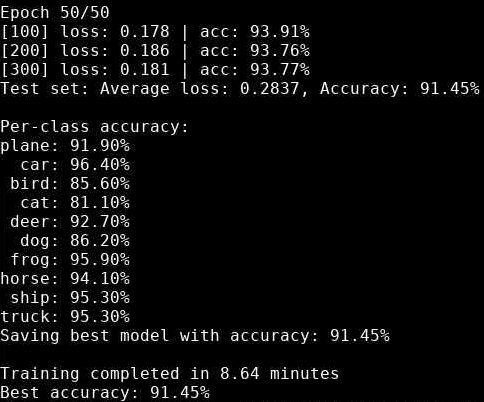
\includegraphics[width=0.9\textwidth]{media/cnn_sgd_epoch_50.png}
            \vspace{-0.3cm}
            \caption{SGD: Last Epoch}
        \end{figure}
    \end{column}
\end{columns}
\end{frame}

\begin{frame}
\frametitle{Normalization value Variations}
\begin{columns}
    \begin{column}{0.4\textwidth}
        \begin{figure}[t]
            \centering
            \vspace{-0.4cm}
            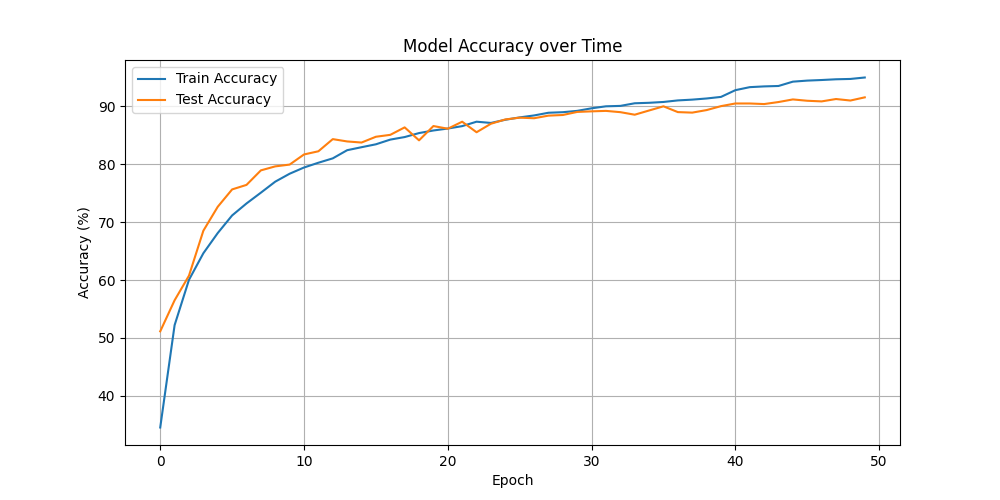
\includegraphics[width=0.9\textwidth]{media/cifar10_cnn_accuracy.png}
        \end{figure}
        \vspace{-0.6cm}
        \begin{figure}[t]
            \centering
            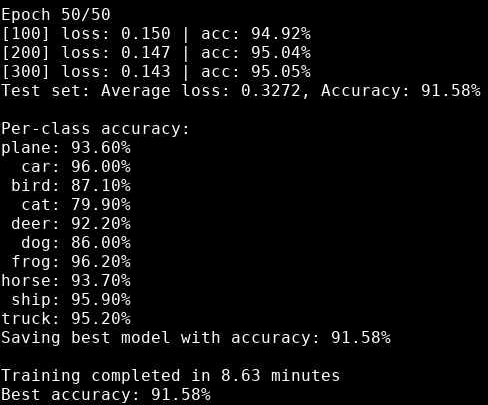
\includegraphics[width=0.9\textwidth]{media/cnn_epoch_50.png}
            \vspace{-0.3cm}
            \caption{Optimized}
        \end{figure}
        Mean: (0.4914, 0.4822, 0.4465),\\
        Standard Deviation: (0.2023, 0.1994, 0.2010)
    \end{column}

    \begin{column}{0.4\textwidth}
        \begin{figure}[t]
            \centering
            \vspace{-0.4cm}
            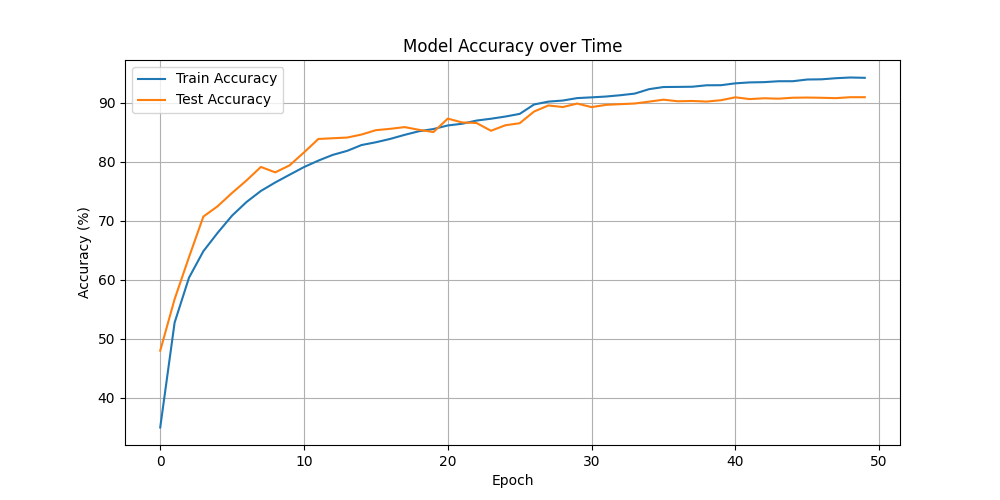
\includegraphics[width=0.9\textwidth]{media/cifar10_cnn_std_accuracy.png}
        \end{figure}
        \vspace{-0.6cm}
        \begin{figure}[t]
            \centering
            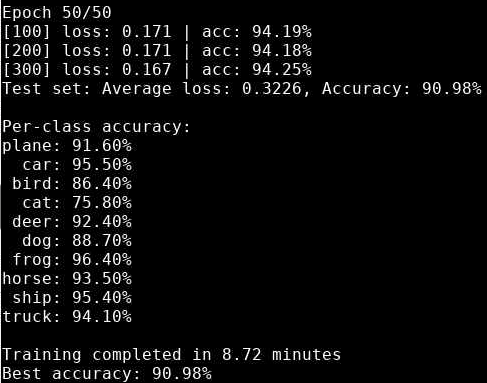
\includegraphics[width=0.9\textwidth]{media/cnn_std_epoch_50.png}
            \vspace{-0.3cm}
            \caption{Standard}
        \end{figure}
        Mean: (0.5, 0.5, 0.5),\\
        Standard Deviation: (0.5, 0.5, 0.5)
    \end{column}

    \begin{column}{0.4\textwidth}
        \begin{figure}[t]
            \centering
            \vspace{-0.4cm}
            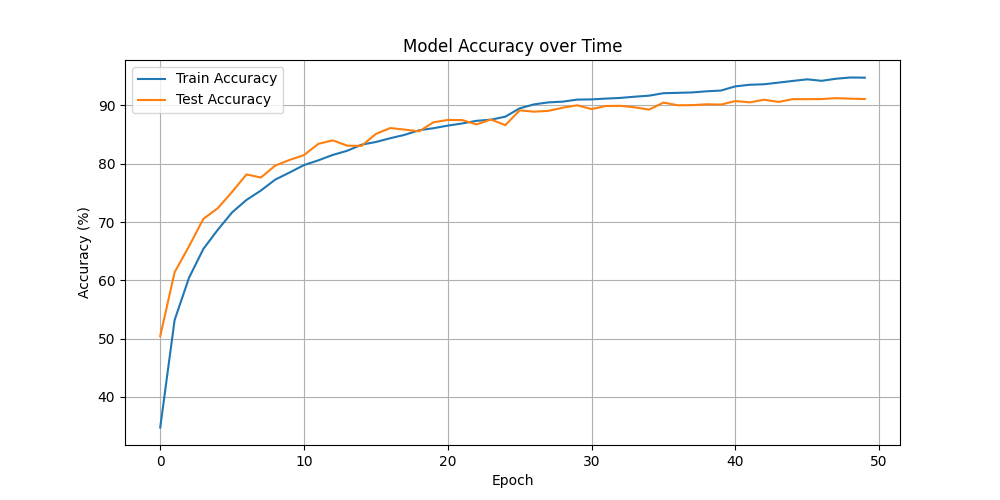
\includegraphics[width=0.9\textwidth]{media/cifar10_cnn_zero_accuracy.png}
        \end{figure}
        \vspace{-0.6cm}
        \begin{figure}[t]
            \centering
            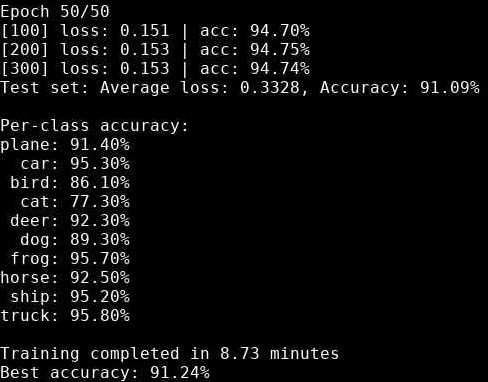
\includegraphics[width=0.9\textwidth]{media/cnn_zero_epoch_50.png}
            \vspace{-0.3cm}
            \caption{Zero-centered}
        \end{figure}
        Mean: (0.5, 0.5, 0.5),\\
        Standard Deviation: (0.25, 0.25, 0.25)
    \end{column}
\end{columns}
\end{frame}
\end{document}